%MULTIPLICATION ON A NUMBER LINE - WORKSHEET 0 (IN-CLASS INSTRUCTION)
\documentclass[12pt, letterpaper, fleqn]{article}

% ----------------------------------------------------------
% PACKAGES
% ----------------------------------------------------------
\usepackage{graphicx}
\usepackage{xcolor}
\usepackage[most]{tcolorbox}
\usepackage{amsmath, amssymb}
\usepackage{fancyhdr}
\usepackage[utf8]{inputenc}
\usepackage[T1]{fontenc}
\usepackage{enumitem}
\usepackage{geometry}
\usepackage{tikz}
\usepackage{needspace}
\usepackage{multicol}

\usetikzlibrary{arrows.meta, calc, shapes.geometric}

% ----------------------------------------------------------
% PAGE SETUP
% ----------------------------------------------------------
\usepackage{times}
\geometry{letterpaper, top=1.25in, bottom=1.25in, marginpar=0.5in}

% ----------------------------------------------------------
% HEADER / FOOTER
% ----------------------------------------------------------
\newcommand{\logowidth}{3cm}
\setlength{\headheight}{20pt}
\setlength{\footskip}{40pt}

\pagestyle{fancy}
\fancyhf{}
\fancyhead[C]{\small\bfseries Multiplication on a Number Line}
\fancyfoot[L]{\raisebox{2pt}{
\includegraphics[width=\logowidth]{../kss.png}}}
\fancyfoot[C]{\thepage}
\fancyfoot[R]{3.2.0}

\renewcommand{\footrulewidth}{0.2pt}

% ----------------------------------------------------------
% THEME COLOR
% ----------------------------------------------------------
\definecolor{customteal}{HTML}{2fbdb9}

% ----------------------------------------------------------
% HELPER MACROS
% ----------------------------------------------------------
\newcommand{\blank}{\underline{\hspace{2.2cm}}}
\newcommand{\blanklong}{\underline{\hspace{6.5cm}}}
\newcommand{\blankshorter}{\underline{\hspace{1.5cm}}}

% ----------------------------------------------------------
% DOCUMENT
% ----------------------------------------------------------
\begin{document}

\textbf{Name:} \underline{\hspace{5cm}}
\hfill
\textbf{Date:} \underline{\hspace{3cm}}\\

\begin{tcolorbox}[colback=customteal!20]
    \large\textcolor{black}{\textbf{Multiplication on a Number Line}}
\end{tcolorbox}

\vspace{3mm}
\noindent
We can model multiplication as **equal jumps** on a number line.
\begin{center}
\begin{tikzpicture}[scale=0.9]
\draw[latex-latex, thick] (-0.5,0) -- (10.5,0);
\foreach \x in {0,1,2,3,4,5,6,7,8,9,10} {
  \draw[thick] (\x, 0.1) -- (\x, -0.1) node[below] {\x};
}
% Draw jumps of 2
\draw[->, red, thick] (0,0) to[out=45,in=135] (2,0);
\draw[->, red, thick] (2,0) to[out=45,in=135] (4,0);
\draw[->, red, thick] (4,0) to[out=45,in=135] (6,0);
\draw[->, red, thick] (6,0) to[out=45,in=135] (8,0);
\node at (4, 0.8) {4 jumps of 2};
\end{tikzpicture}
\end{center}
Here, we made **4 jumps** of size **2**. We landed on **8**.
\[
4 \times 2 = 8
\]

\newpage
\begin{tcolorbox}[colback=customteal!20]
    \large\textcolor{black}{\textbf{Guided Practice: Number Lines}}
\end{tcolorbox}

\vspace{5mm}
\noindent
Write the multiplication equation shown by the jumps on each number line.

\vspace{8mm}
\begin{enumerate}[itemsep=3.5cm, leftmargin=0.6cm]
\item 
\begin{tikzpicture}[scale=0.9]
\draw[latex-latex, thick] (-0.5,0) -- (10.5,0);
\foreach \x in {0,1,2,3,4,5,6,7,8,9,10} {
  \draw[thick] (\x, 0.1) -- (\x, -0.1) node[below] {\x};
}
\draw[->, blue, thick] (0,0) to[out=45,in=135] (3,0);
\draw[->, blue, thick] (3,0) to[out=45,in=135] (6,0);
\draw[->, blue, thick] (6,0) to[out=45,in=135] (9,0);
\end{tikzpicture}
\\
Equation: \blank $\times$ \blank $=$ \blank

\item 
\begin{tikzpicture}[scale=0.9]
\draw[latex-latex, thick] (-0.5,0) -- (10.5,0);
\foreach \x in {0,1,2,3,4,5,6,7,8,9,10} {
  \draw[thick] (\x, 0.1) -- (\x, -0.1) node[below] {\x};
}
\draw[->, orange, thick] (0,0) to[out=45,in=135] (5,0);
\draw[->, orange, thick] (5,0) to[out=45,in=135] (10,0);
\end{tikzpicture}
\\
Equation: \blank $\times$ \blank $=$ \blank
\end{enumerate}

\end{document}
